\documentclass{clbeamer2024}

\usepackage{minted}

\usepackage{minted}
\setminted{
	breaklines=true,
	frame=single,
	bgcolor=lightgray,
	fontsize=\small,
	escapeinside=||
}

\usepackage{xcolor}
\definecolor{bg}{rgb}{0.95, 0.95, 0.92} % Couleur gris clair

\title{
	%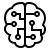
\includegraphics[width=0.5cm]{logos/IA1.png} \hfill
        Introduction à la Complexité
	
\includegraphics[width=0.7cm]{logos/complexity.png} \hfill
}
\subtitle{Comprendre les bases de la théorie de la complexité}
\author{Slimani Mohamed Amine}
\institute{EHTP}
\date{\today}

\begin{document}
	\setcounter{framenumber}{-1}
	\frame{\titlepage}
	
	
	
	% Sommaire
	\begin{frame}{Sommaire}
		\tableofcontents
	\end{frame}
	
	
	\section{Qu'est-ce que la complexité ?}
	\begin{frame}{Qu'est-ce que la complexité ?}
		\begin{itemize}
			\item \textbf{Définition} : La complexité est une mesure des ressources nécessaires pour résoudre un problème, souvent en termes de temps et d'espace.
			\item \textbf{Objectif} : Évaluer l'efficacité des algorithmes et comprendre les limites de la calculabilité.
			\item \textbf{Avantages} : Permet de comparer des algorithmes et de prédire leur comportement sur de grandes entrées.
		\end{itemize}
	\end{frame}
	
	\section{Pourquoi étudier la complexité ?}
	\begin{frame}{Pourquoi étudier la complexité ?}
		\begin{itemize}
			\item \textbf{Optimisation} : Identifier les algorithmes les plus efficaces pour un problème donné.
			\item \textbf{Prédiction} : Anticiper les performances des algorithmes sur de grandes entrées.
			\item \textbf{Théorie} : Comprendre les limites fondamentales de ce qui peut être calculé.
		\end{itemize}
	\end{frame}
	
	
	\section{Concepts de base de la complexité}
	\begin{frame}{Concepts de base de la complexité}
		\begin{itemize}
			\item \textbf{Complexité en temps} : Nombre d'étapes nécessaires pour résoudre un problème.
			\item \textbf{Complexité en espace} : Quantité de mémoire nécessaire pour résoudre un problème.
			\item \textbf{Notation Big-O} : Utilisée pour décrire la croissance asymptotique d'une fonction.
		\end{itemize}
	\end{frame}
	
\section{Classes de complexité}
\begin{frame}{Classes de complexité}
	\begin{center}
		\begin{tabular}{|c|c|}
			\hline
			\textbf{O} & \textbf{Type de complexité} \\
			\hline
			\(O(1)\) & Constante \\
			\hline
			\(O(\log(n))\) & Logarithmique \\
			\hline
			\(O(n)\) & Linéaire \\
			\hline
			\(O(n \times \log(n))\) & Quasi-linéaire \\
			\hline
			\(O(n^2)\) & Quadratique \\
			\hline
			\(O(n^3)\) & Cubique \\
			\hline
			\(O(2^n)\) & Exponentielle \\
			\hline
			\(O(n!)\) & Factorielle \\
			\hline
		\end{tabular}
	\end{center}
\end{frame}


\section{Exemple d'analyse de complexité}
\begin{frame}{Exemple d'analyse de complexité}
	\begin{exampleblock}{Analyse de complexité}
		\begin{center}
			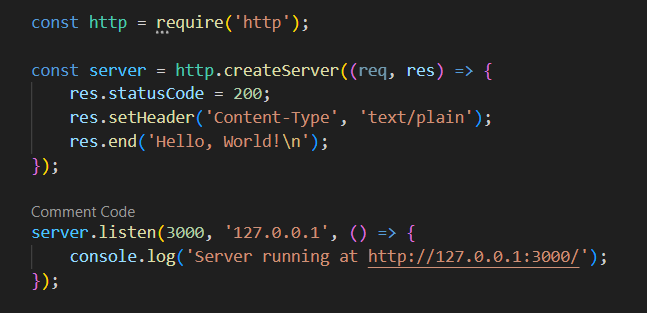
\includegraphics[width=0.7\textwidth]{images/code1.png}
		\end{center}
	
	\end{exampleblock}
\end{frame}


\section{Bonnes pratiques}
\begin{frame}{Bonnes pratiques}
	\begin{itemize}
		\item \textbf{Choix d'algorithmes} : Préférer les algorithmes avec une complexité en temps et espace optimale.
		\item \textbf{Analyse} : Toujours analyser la complexité avant de choisir un algorithme.
		\item \textbf{Optimisation} : Éviter les optimisations prématurées sans comprendre la complexité.
	\end{itemize}
\end{frame}


\section{Outils pour analyser la complexité}
\begin{frame}{Outils pour analyser la complexité}
	\begin{itemize}
		\item \textbf{Profiling} : Utiliser des outils de profiling pour mesurer les performances.
		\item \textbf{Simulation} : Simuler des entrées de grande taille pour prédire le comportement.
		\item \textbf{Théorie} : Étudier la théorie de la complexité pour mieux comprendre les limites.
	\end{itemize}
\end{frame}


\section{Exemple d'application avec Python}
\begin{frame}{Exemple d'application avec Python}
	\begin{exampleblock}{Analyse de complexité en Python}
		
		\begin{center}
			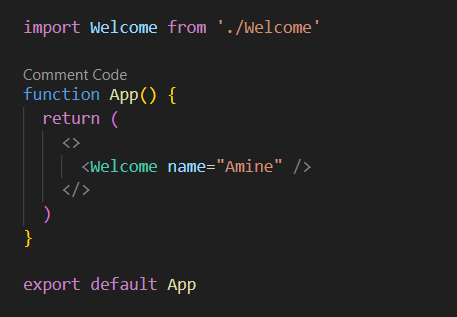
\includegraphics[width=0.7\textwidth]{images/code2.png}
		\end{center}
		
	\end{exampleblock}
\end{frame}


\section{Défis de la complexité}
\begin{frame}{Défis de la complexité}
	\begin{itemize}
		\item \textbf{Problèmes NP-Complets} : Résoudre ces problèmes de manière efficace reste un défi.
		\item \textbf{Grandes entrées} : Les algorithmes peuvent devenir inefficaces sur de très grandes entrées.
		\item \textbf{Optimisation} : Trouver un équilibre entre temps et espace peut être difficile.
	\end{itemize}
\end{frame}

\section{Pourquoi c'est important ?}
\begin{frame}{Pourquoi c'est important ?}
	\begin{itemize}
		\item La complexité est essentielle pour comprendre les limites des algorithmes.
		\item Elle permet de choisir les meilleurs algorithmes pour des problèmes spécifiques.
		\item Comprendre la complexité est crucial pour les développeurs et les chercheurs en informatique.
	\end{itemize}
\end{frame}

\begin{frame}{Résumé}
	\textbf{La complexité} est un concept fondamental en informatique pour comprendre et optimiser les algorithmes.  
	Explorez, apprenez, et innovez avec la théorie de la complexité !
\end{frame}


	
\end{document}
